\documentclass[11pt, letterpaper]{article}
\usepackage[utf8]{inputenc}
\usepackage{graphicx}
\usepackage{indentfirst}
\usepackage{float}
\setlength{\parindent}{5ex}


\usepackage{geometry}
\usepackage{booktabs}
 \geometry{
 letterpaper,
 left=1.2in,
 top=1in,
 right=1.2in,
 bottom=1.1in,
 }

\begin{document}

\begin{titlepage}
    \begin{center}
        \vspace*{1cm}

        \Huge
        \textbf{Voltage Controller Manual}

        \vspace{0.5cm}
        \LARGE

        \vspace{1.5cm}

        \textbf{Alexander Fogal}

        \vspace{7.8cm}

        \Large
        For Professor Jim Martin\\
        University of Waterloo\\
        August 9th, 2021

    \end{center}
\end{titlepage}

\tableofcontents

\newpage

\section{Setup}
\subsection{Rasbperry Pi}
To setup the Raspberry Pi:

\begin{enumerate}
    \item Unplug Ethernet and Power from RPi if plugged in, and move to desired location
    \item If the DAC/ADC board was unplugged, plug it in now. Make sure the wire with the red striping is aligned with pin 1 on the RPi. Make sure the plug is aligned with the pins properly and BEFORE powering the RPi (or else the control software will fail since the i2c isn't connected)
    \item Plug in ethernet and power to RPi and allow it about a minute to finish booting
\end{enumerate}

\subsection{Remote Setup}
To setup your personal computer or a lab computer:
\begin{enumerate}
    \item Clone the github repo
    \item Install dependencies:
    \begin{verbatim}
        sudo apt install python3 python3-paho-mqtt python3-pyqt5
    \end{verbatim}
    \item This is only necessary in theory or as a check since I have setup the RPi to use the static IP \verb|192.168.1.4| and I have \verb|mosquitto| running on the Pi at boot.
    \begin{enumerate}
        \item On a laptop/desktop (or even the Pi itself if plugged into a display), run \verb|ip addr| to find your IP address as pictured (see Figure 1 at the end of the document). Then run \verb|nmap| as pictured as well. Note that the Pi and control computer must be plugged into the same router. Make sure the address in the nmap command is the same as your IP address but with a zero in the final entry (and leave the /24).
        \item The IP of the RPi will be labelled as in the picture
        \item Change the IP in the defaultSettings dictionary in server/server.py to the IP of the RPi found in nmap.
    \end{enumerate}
    \item Now you should be able to run \verb|python3 server.py| and have everything connect! It will take a moment, but it should not take more than 30 seconds.
    \item If not, the relevant ssh command is:
        \begin{verbatim}
            ssh -l jddmartin RPi_IP_Here 
        \end{verbatim}
    Ask Jim or I for the password. Feel free to message me if it isn't working as expected!

\end{enumerate}
\newpage

\begin{figure}[H]
    \centering
    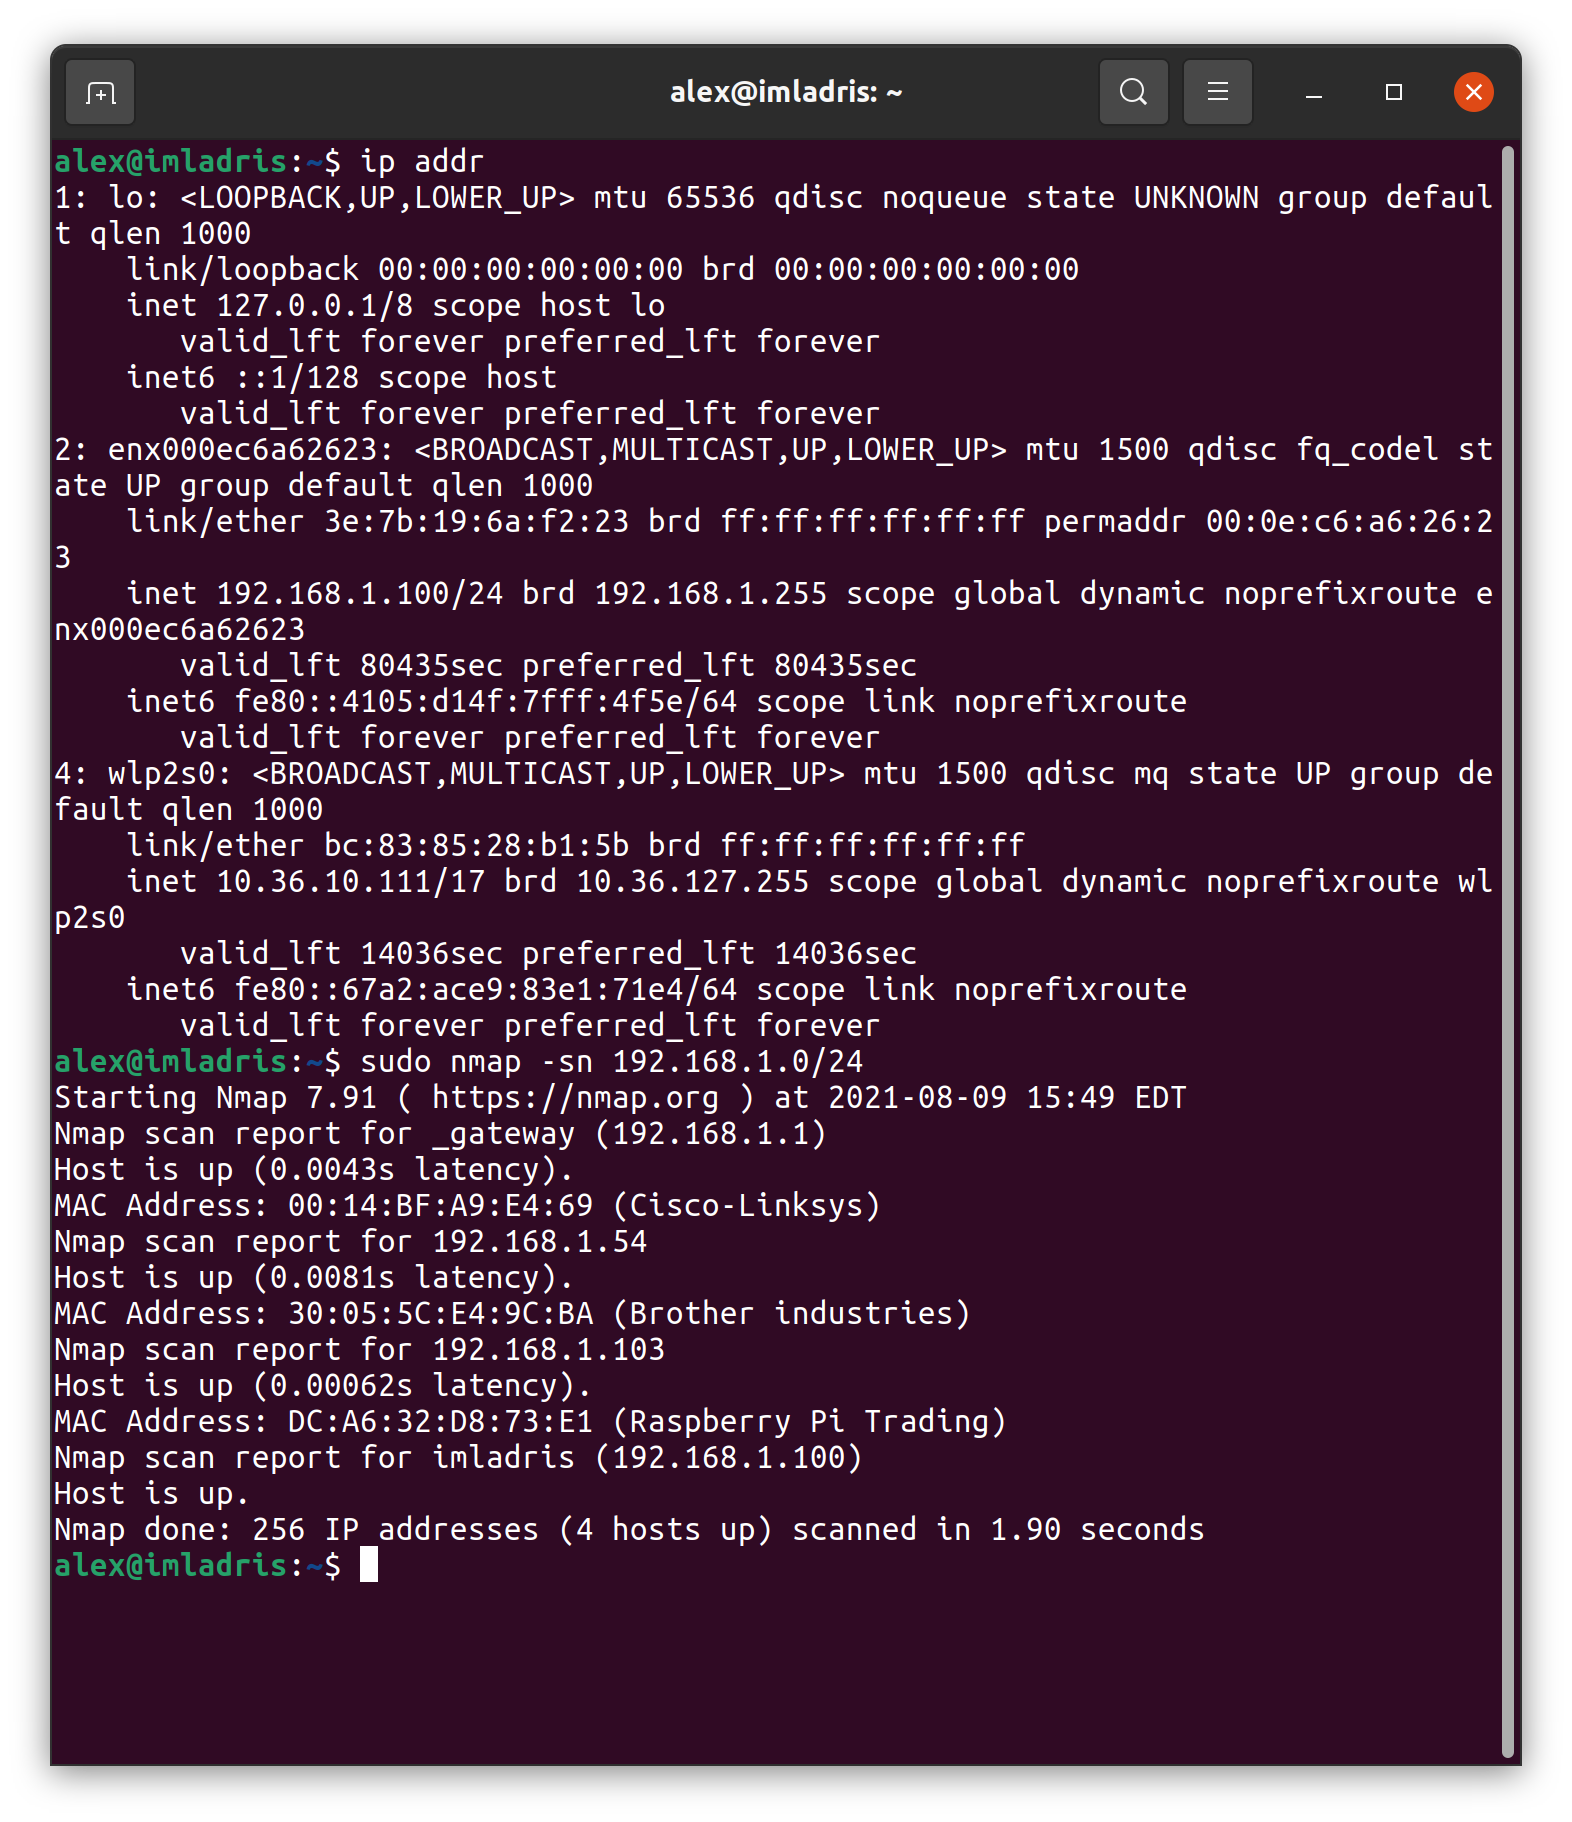
\includegraphics[width=17cm]{find_ip.png}
    \caption{ Commands to check your IP and find the IP of the RPi. If you are using ethernet, the relevant interface will be either enx... or eth0. Otherwise, for WiFi it will be either wlp... or wlan0. In this case, I am using ethernet and so my IP can be read (next to inet) as 192.168.1.100. Further, note that the relevant IP for a name is {\it above} it, i.e., the IP for the RPi in this picture is 192.168.1.103.}
    \label{fig:find_ip}
\end{figure}
\section{Interface}
The interface is rather simple:
\begin{figure}[H]
    \centering
    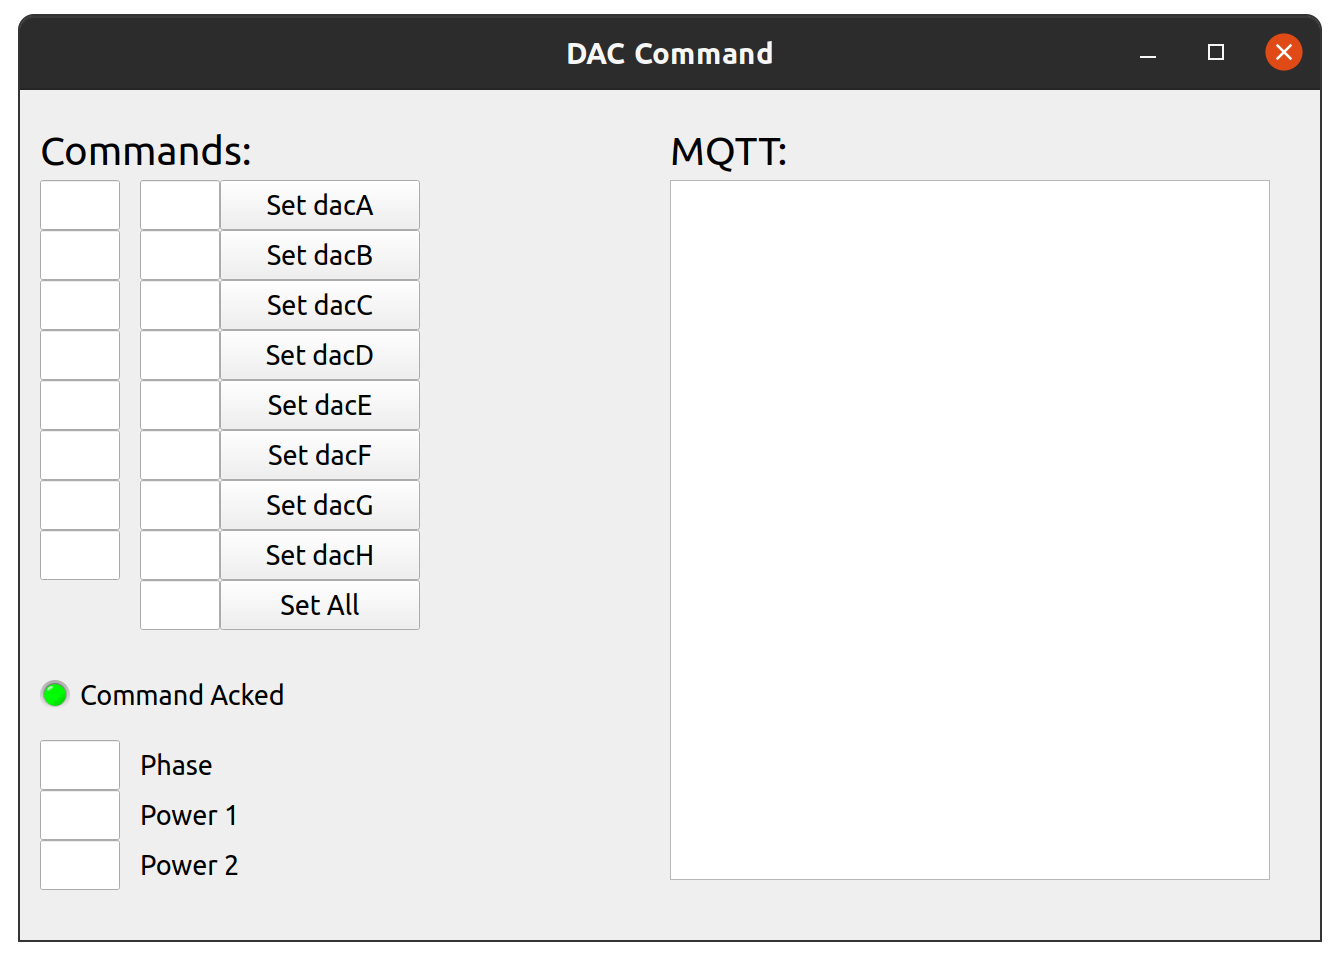
\includegraphics[width=16cm]{command_ui.png}
    \caption{ Command UI for the DAC/ADC board. The left column of text boxes report the current state of the DACs, the right column is for setting the DACs. The bottom section are ADC readouts. MQTT messages will appear in the box to the right.  }
    \label{fig:command_ui}
\end{figure}

In order to set the DACs, one can simply enter a value and click the relevant set button. Errors will occur if there was trouble converting the string to a float value, which will be reported in the MQTT box as well. Values should be between 0 and 5V. The board looks like this:

\begin{figure}[H]
    \centering
    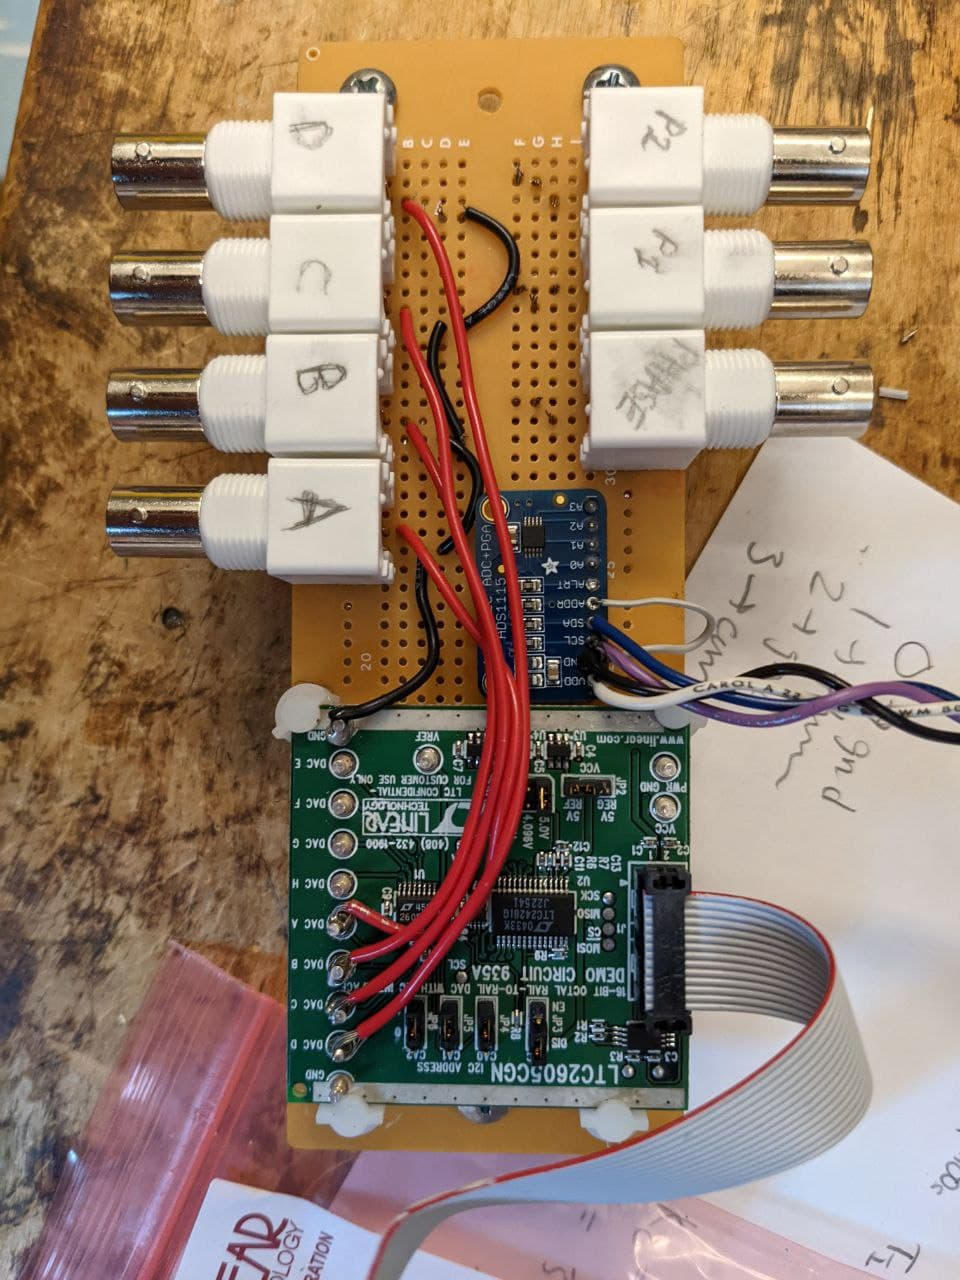
\includegraphics[width=16cm]{board.jpg}
    \caption{ DAC/ADC board, DAC BNCs are labelled and ADC BNCs are labelled, both done rather crudely. }
    \label{fig:board}
\end{figure}




\end{document}